\documentclass{article}
\usepackage{amsmath, amssymb, amsthm}
\usepackage{tikz}
\usepackage{listings}
\usepackage{hyperref}
\usepackage[margin=1in]{geometry}
\usepackage{xcolor}

\usetikzlibrary{calc, arrows.meta, decorations.pathmorphing, 3d}

\definecolor{codebg}{RGB}{245,245,245}
\definecolor{codekw}{RGB}{170,40,170}
\definecolor{codestr}{RGB}{40,120,40}
\definecolor{codecmt}{RGB}{120,120,120}

\lstset{
  backgroundcolor=\color{codebg},
  basicstyle=\ttfamily\small,
  keywordstyle=\color{codekw}\bfseries,
  stringstyle=\color{codestr},
  commentstyle=\color{codecmt}\itshape,
  showstringspaces=false,
  breaklines=true,
  frame=single,
  framerule=0pt,
  xleftmargin=8pt,
  xrightmargin=8pt
}

\title{Guide 16: Equirectangular Projection and Spherical Coordinates}
\author{web-3d-panel-navigation math curriculum}
\date{}

\begin{document}
\maketitle

\section{Why this matters}

Open \texttt{src/skybox/panorama-skybox.ts} and look at line 25:

\begin{lstlisting}[language=JavaScript]
loaded.mapping = THREE.EquirectangularReflectionMapping;
loaded.colorSpace = THREE.SRGBColorSpace;
\end{lstlisting}

Two assignments. Two lines. Yet they are the entire reason a user can hand the
panel-navigation library a single 4096$\times$2048 JPEG of, say, a cathedral
interior, and have that cathedral wrap seamlessly around the 3D scene as the
sky behind the panels. The flat photo becomes a sphere. No 3D modelling, no
six-image cube, just a 2:1 rectangle and a one-line tag that tells Three.js
``treat this as a panorama.''

That is a remarkable amount of leverage from a tiny piece of API, and behind
it is a piece of math worth understanding. The \emph{equirectangular
projection} is how a 2D image gets to be a sphere's surface. It is also,
crucially, a \emph{lossy} mapping: it stretches things at the poles in a
predictable way, and that distortion is a Jacobian we have already met in
guide 15. This guide closes the curriculum by tying spherical coordinates,
projection geometry, the polar pinch, and Three.js's texture-mapping API
together into one final picture.

\section{Building intuition}

Imagine standing inside a glass sphere and painting longitude and latitude
lines on the inside. Meridians (lines of constant longitude $\phi$) all run
from the north pole through the equator down to the south pole. Parallels
(lines of constant latitude) are horizontal circles that shrink as you go
toward either pole.

\begin{center}
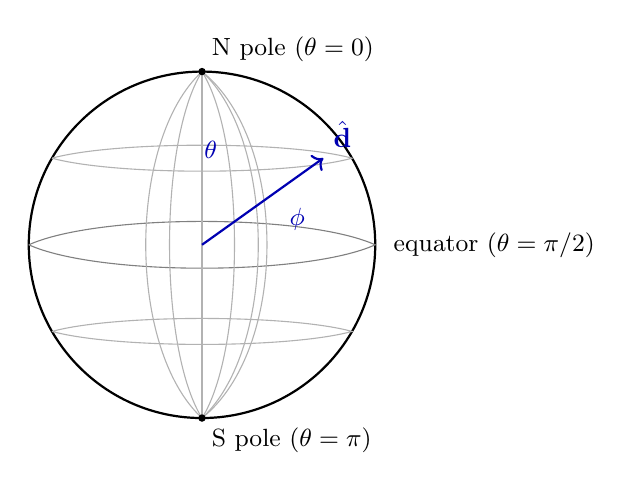
\begin{tikzpicture}[scale=2.2]
  % Sphere outline
  \draw[thick] (0,0) circle (1);
  % Equator (perspective ellipse)
  \draw[gray] (-1,0) .. controls (-0.6,-0.18) and (0.6,-0.18) .. (1,0)
                     .. controls (0.6,0.18)  and (-0.6,0.18)  .. (-1,0);
  % Parallels above/below
  \draw[gray!60] (-0.866,0.5) .. controls (-0.5,0.4) and (0.5,0.4) .. (0.866,0.5)
                              .. controls (0.5,0.6) and (-0.5,0.6) .. (-0.866,0.5);
  \draw[gray!60] (-0.866,-0.5) .. controls (-0.5,-0.6) and (0.5,-0.6) .. (0.866,-0.5)
                               .. controls (0.5,-0.4) and (-0.5,-0.4) .. (-0.866,-0.5);
  % Meridians
  \foreach \a in {0, 30, 60, 90, 120, 150} {
    \draw[gray!60] (0,1) .. controls ({0.5*cos(\a)},{0.6}) and ({0.5*cos(\a)},{-0.6}) .. (0,-1);
  }
  % Poles
  \filldraw (0,1) circle (0.018) node[above right] {\small N pole ($\theta=0$)};
  \filldraw (0,-1) circle (0.018) node[below right] {\small S pole ($\theta=\pi$)};
  % Labels
  \node[right] at (1.05,0) {\small equator ($\theta=\pi/2$)};
  \draw[->, thick, blue!70!black] (0,0) -- (0.7,0.5) node[above right] {$\hat{\mathbf{d}}$};
  \node[blue!70!black] at (0.55,0.15) {\small $\phi$};
  \node[blue!70!black] at (0.05,0.55) {\small $\theta$};
\end{tikzpicture}
\end{center}

Now ``cut'' this sphere along the prime meridian, peel it off, and lay it
flat. The meridians, which were converging at the poles, become vertical
lines. The parallels become horizontal lines. To make this rectangle fit, the
top and bottom rows have to be stretched horizontally to match the equator's
length. That stretch is the equirectangular projection:

\begin{center}
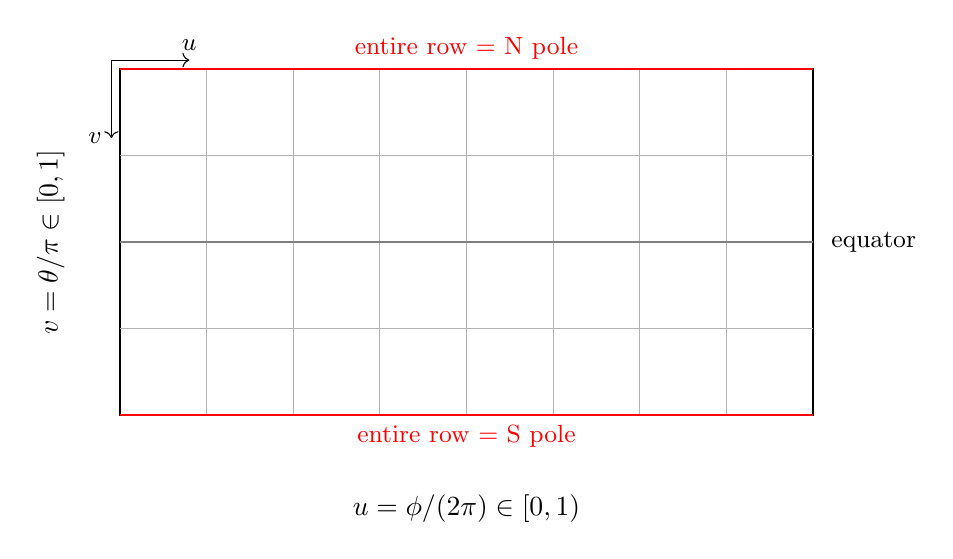
\begin{tikzpicture}[scale=2.2]
  % 2:1 rectangle
  \draw[thick] (0,0) rectangle (4,2);
  % Vertical grid (meridians)
  \foreach \x in {0.5, 1.0, 1.5, 2.0, 2.5, 3.0, 3.5} {
    \draw[gray!60] (\x,0) -- (\x,2);
  }
  % Horizontal grid (parallels)
  \foreach \y in {0.5, 1.0, 1.5} {
    \draw[gray!60] (0,\y) -- (4,\y);
  }
  % Bold equator
  \draw[thick, gray] (0,1) -- (4,1);
  \node[right] at (4.05,1) {\small equator};
  % Pole rows
  \draw[red, thick] (0,2) -- (4,2);
  \draw[red, thick] (0,0) -- (4,0);
  \node[red, above] at (2,2) {\small entire row $=$ N pole};
  \node[red, below] at (2,0) {\small entire row $=$ S pole};
  % Axis labels
  \node[below] at (2,-0.4) {$u = \phi/(2\pi) \in [0,1)$};
  \node[left, rotate=90, anchor=center] at (-0.4,1) {$v = \theta/\pi \in [0,1]$};
  \draw[->] (-0.05,2.05) -- (0.4,2.05) node[above] {\small $u$};
  \draw[->] (-0.05,2.05) -- (-0.05,1.6) node[left] {\small $v$};
\end{tikzpicture}
\end{center}

Notice the red top and bottom edges. On the sphere, those collapse to
\emph{single points} (the poles). On the flat map, they are entire rows of
pixels. That redundancy is the price the projection pays to be rectangular.

Here is the same idea drawn as a polar pinch: take a square texel near the
equator and a square texel near the pole. The first covers a normal patch of
sphere; the second covers a sliver, because all the meridians are
crowding together.

\begin{center}
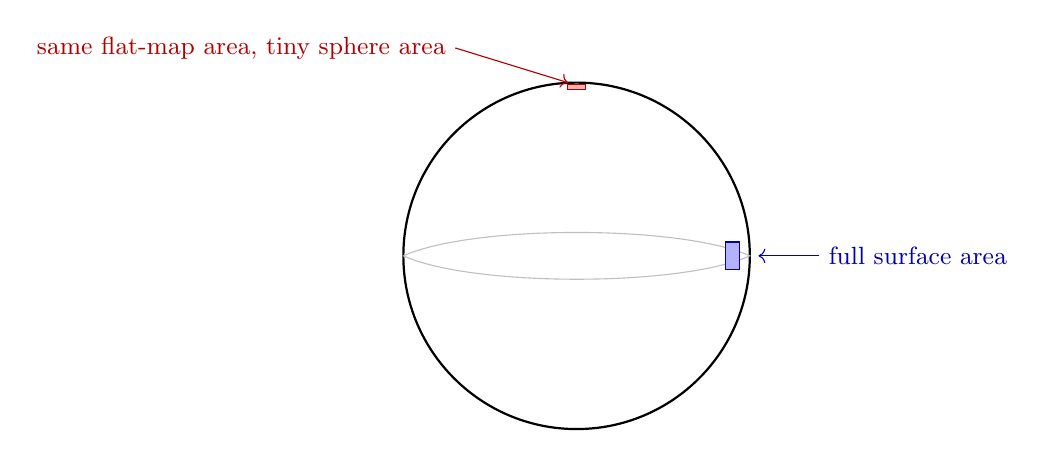
\begin{tikzpicture}[scale=2.2]
  % Sphere
  \draw[thick] (0,0) circle (1);
  \draw[gray!50] (-1,0) .. controls (-0.6,-0.18) and (0.6,-0.18) .. (1,0)
                        .. controls (0.6,0.18)  and (-0.6,0.18)  .. (-1,0);
  % Equator patch (a "square" in (theta, phi) near theta=pi/2)
  \filldraw[blue!30, draw=blue!70!black] (0.94,-0.08) -- (0.94,0.08) -- (0.86,0.08) -- (0.86,-0.08) -- cycle;
  \draw[->, blue!70!black] (1.4,0) -- (1.05,0);
  \node[right, blue!70!black] at (1.4,0) {\small full surface area};
  % Pole patch (a "square" near theta near 0)
  \filldraw[red!30, draw=red!70!black] (-0.05,0.96) -- (0.05,0.96) -- (0.05,0.99) -- (-0.05,0.99) -- cycle;
  \draw[->, red!70!black] (-0.7,1.2) -- (-0.05,1.0);
  \node[left, red!70!black] at (-0.7,1.2) {\small same flat-map area, tiny sphere area};
\end{tikzpicture}
\end{center}

The Jacobian we are about to derive is exactly $\sin\theta$: it goes to 1 at
the equator and to 0 at the poles, which is the formal statement of that
pinch.

\section{The math}

\subsection{Spherical coordinates}

A point on the unit sphere is parameterised by polar angle
$\theta \in [0, \pi]$ measured from the north pole and azimuth
$\phi \in [0, 2\pi)$ measured around the vertical axis:
\begin{equation}
  \mathbf{p}(\theta, \phi) = \begin{pmatrix} \sin\theta\,\cos\phi \\ \sin\theta\,\sin\phi \\ \cos\theta \end{pmatrix}.
\end{equation}
At $\theta = 0$ the point is the north pole $(0, 0, 1)$ regardless of $\phi$;
at $\theta = \pi$ it is the south pole $(0, 0, -1)$. The equator is the
circle at $\theta = \pi/2$.

To match geographic conventions you sometimes see latitude
$\beta = \pi/2 - \theta$ and longitude $\lambda = \phi$, but Three.js's
\texttt{EquirectangularReflectionMapping} works directly with the polar form,
so we will stick with $(\theta, \phi)$.

\subsection{The equirectangular projection}

Define texture coordinates $(u, v)$ with $u$ horizontal, $v$ vertical, and the
image-standard convention that $v = 0$ is the top of the image. The
equirectangular map is the simplest possible:
\begin{equation}
  (\theta, \phi) \longmapsto (u, v) = \left( \frac{\phi}{2\pi}, \; \frac{\theta}{\pi} \right),
  \qquad u \in [0, 1), \; v \in [0, 1].
\end{equation}
Its inverse:
\begin{equation}
  (u, v) \longmapsto (\theta, \phi) = (\pi v, \; 2\pi u).
\end{equation}
The image domain has width $2\pi$ (one full loop around) and height $\pi$ (north
pole to south pole). The aspect ratio is exactly 2:1 --- this is why
panoramas are 4096$\times$2048, 8192$\times$4096, and so on.

\subsection{The Jacobian and the polar pinch}

From guide 15, the differential surface area on the unit sphere is
\begin{equation}
  dA_{\text{sphere}} = \sin\theta \; d\theta \, d\phi.
\end{equation}
Differential area on the equirectangular flat map, in the underlying
$(\phi, \theta)$ measure, is just
\begin{equation}
  dA_{\text{flat}} = d\phi \, d\theta = (2\pi \, du)(\pi \, dv) = 2\pi^2 \, du \, dv.
\end{equation}
The ratio is the Jacobian:
\begin{equation}
  \boxed{\frac{dA_{\text{sphere}}}{d\theta \, d\phi} = \sin\theta.}
\end{equation}
At the equator ($\theta = \pi/2$), $\sin\theta = 1$ --- maximal sphere area
per flat-map cell. At either pole ($\theta \to 0$ or $\theta \to \pi$),
$\sin\theta \to 0$ --- a flat-map cell maps to vanishing surface area. This
is the polar pinch in one symbol.

\subsection{Connection to guide 15: uniform sampling is not just $(u, v)$}

A naive instinct would be: ``to put random stars on the sky, pick uniform
random $u, v \in [0, 1)$, convert to $(\theta, \phi)$, place a star.'' But by
the Jacobian above, that recipe gives more stars per unit \emph{flat-map
area}, which translates to more stars per unit \emph{$d\theta \, d\phi$},
which is \emph{not} the same as more stars per unit $dA_{\text{sphere}}$. The
result clusters at the poles. Guide 15's correction --- sample
$z = 2u_1 - 1$ uniformly and $\phi = 2\pi u_2$ uniformly --- is precisely the
inverse-CDF construction that absorbs the $\sin\theta$ factor. Equirectangular
makes this very concrete: it is the mapping whose Jacobian we are correcting.

\subsection{Three.js's role}

You do not write the mapping yourself. Inside the GPU shader, Three.js takes
the fragment's world-space surface direction $\hat{\mathbf{d}} = (x, y, z)$
on a unit sphere and computes
\begin{equation}
  \theta = \arccos(y), \qquad \phi = \mathrm{atan2}(z, x),
\end{equation}
then maps to UV. (The $y$-up axis convention is Three.js's; $\theta$ is taken
from the up axis.) Your only responsibility, on the JS side, is to tag the
texture with the right \texttt{mapping} so the shader uses this code path,
and the right \texttt{colorSpace} so the colours decode correctly. Both
assignments live on the texture object after loading:

\begin{lstlisting}[language=JavaScript]
loaded.mapping = THREE.EquirectangularReflectionMapping;
loaded.colorSpace = THREE.SRGBColorSpace;
\end{lstlisting}

\subsection{The pole singularity}

The map $(u, v) \to (\theta, \phi) = (\pi v, 2\pi u)$ is one-to-one on the
open square $(0, 1) \times (0, 1)$ but is degenerate at $v = 0$ and $v = 1$.
At $v = 0$ every $u$ produces the same point $(0, 1, 0)$, the north pole;
at $v = 1$ every $u$ produces the south pole. The flat image stores $W$
distinct pixels along the top edge that all represent one sphere point. This
causes filtering artifacts at the poles in low-quality panoramas: blurring,
banding, sometimes a visible ``swirl.''

If you need to avoid this, you switch projection. Cubemaps split the sphere
into six square faces with no polar singularity. The project supports them
through \texttt{createImageSkybox} in \texttt{src/skybox/image-skybox.ts}:
six images, no pole pinch, but six images to author. There are also
equiangular cubemaps and dual-fisheye projections used in 360-video
production; the trade-off is always between authoring simplicity and pole
quality.

\subsection{Color space, briefly}

Image files almost always store color values in sRGB encoding, which is
roughly a $\gamma \approx 2.2$ power curve so that an 8-bit channel
distributes its 256 values in a perceptually uniform way (more codes near
black, where the eye is more sensitive). A GPU doing lighting math wants
\emph{linear-light} values: doubling a number should double the radiance.
Tagging the texture \texttt{SRGBColorSpace} tells Three.js to insert the
inverse-gamma decode in the shader so blends and lighting happen in linear
space and the final framebuffer is re-encoded for display. Skip this and
your panorama looks washed out and overly bright in the midtones.

\section{In this codebase}

Below is the full provider:

\begin{lstlisting}[language=JavaScript]
import * as THREE from "three";
import type { Skybox } from "./skybox";

export interface PanoramaSkyboxOptions {
  url: string;
}

export function createPanoramaSkybox(options: PanoramaSkyboxOptions): Skybox {
  const root = new THREE.Group();
  let texture: THREE.Texture | null = null;
  let attachedScene: THREE.Scene | null = null;
  let disposed = false;

  const loader = new THREE.TextureLoader();
  const ready = loader.loadAsync(options.url).then((loaded) => {
    if (disposed) {
      loaded.dispose();
      return;
    }
    loaded.mapping = THREE.EquirectangularReflectionMapping;
    loaded.colorSpace = THREE.SRGBColorSpace;
    texture = loaded;
    if (attachedScene) {
      attachedScene.background = texture;
    }
  });

  return {
    root, ready,
    attach(scene)  { attachedScene = scene; if (texture) scene.background = texture; },
    detach(scene)  { if (scene.background === texture) scene.background = null; attachedScene = null; },
    dispose()      { disposed = true; if (texture) { texture.dispose(); texture = null; } }
  };
}
\end{lstlisting}

The mathematical content is exactly two lines: \texttt{loaded.mapping = THREE.EquirectangularReflectionMapping}
and \texttt{loaded.colorSpace = THREE.SRGBColorSpace}. Everything else is
lifecycle plumbing: load asynchronously, dispose if cancelled, attach to the
scene's \texttt{background} slot when both the texture and a scene are
available. Setting \texttt{scene.background = texture} with the
equirectangular mapping is what causes Three.js's internal renderer to draw
the texture as the infinite-distance sky around all geometry.

The cubemap provider is the same shape:

\begin{lstlisting}[language=JavaScript]
const loader = new THREE.CubeTextureLoader();
const ready = loader.loadAsync(options.cubeUrls).then((loaded) => {
  if (disposed) { loaded.dispose(); return; }
  texture = loaded;
  if (attachedScene) attachedScene.background = texture;
});
\end{lstlisting}

Note the \emph{absence} of a \texttt{mapping} assignment: a
\texttt{CubeTexture} carries its own implicit mapping (lookup by 3D
direction across six faces), so no projection tag is needed. The trade you
are making between the two providers is precisely the trade between
``one image with a pole pinch'' and ``six images with no pole pinch.''

\section{Worked examples}

\subsection*{Example 1: texel area at three latitudes}

Take a 4096$\times$2048 equirectangular image. One texel covers
\[
  \Delta u = \tfrac{1}{4096}, \qquad \Delta v = \tfrac{1}{2048}.
\]
Translating to $(\theta, \phi)$:
\[
  \Delta \phi = 2\pi \, \Delta u = \tfrac{2\pi}{4096}, \qquad
  \Delta \theta = \pi \, \Delta v = \tfrac{\pi}{2048}.
\]
The unit-sphere area covered by that texel at polar angle $\theta$ is
$dA = \sin\theta \, \Delta\theta \, \Delta\phi$. Numerically
$\Delta\theta \, \Delta\phi = \tfrac{2\pi^2}{4096 \cdot 2048} \approx 2.350 \times 10^{-6}$
steradians.

\begin{itemize}
  \item Equator, $\theta = \pi/2$: $\sin\theta = 1$, $dA \approx 2.350 \times 10^{-6}$ sr.
  \item $\theta = \pi/4$ (45$^\circ$ from north pole): $\sin\theta = \tfrac{\sqrt{2}}{2} \approx 0.707$, $dA \approx 1.662 \times 10^{-6}$ sr.
  \item $\theta = \pi/12$ (15$^\circ$ from north pole): $\sin\theta = \sin 15^\circ \approx 0.259$, $dA \approx 6.083 \times 10^{-7}$ sr.
\end{itemize}
At $\theta = \pi/12$ a texel is roughly \emph{a quarter} of an equator texel.
Three or four flat-map texels are doing the work of one equator texel. That
is the visible ``stretching'' near the poles in the source image.

\subsection*{Example 2: world direction $\to$ UV}

Take $\hat{\mathbf{d}} = (1/\sqrt{2}, 0, 1/\sqrt{2})$ in the convention where
$y$ is up. We want $(u, v)$.
\[
  \theta = \arccos(\hat{d}_y) = \arccos(0) = \tfrac{\pi}{2}.
\]
This is the equator: good.
\[
  \phi = \mathrm{atan2}(\hat{d}_z, \hat{d}_x) = \mathrm{atan2}\!\left(\tfrac{1}{\sqrt{2}}, \tfrac{1}{\sqrt{2}}\right) = \tfrac{\pi}{4}.
\]
Then
\[
  u = \frac{\phi}{2\pi} = \frac{1}{8} = 0.125, \qquad v = \frac{\theta}{\pi} = \frac{1}{2} = 0.5.
\]
The fragment samples the panorama at $(0.125, 0.5)$: one-eighth of the way
across, halfway down. On a 4096$\times$2048 image that is pixel $(512, 1024)$.

\subsection*{Example 3: from UV back to direction}

Suppose a star-twinkle effect (guide 14) wants to read what colour the sky is
at $(u, v) = (0.75, 0.25)$.
\[
  \theta = \pi v = \tfrac{\pi}{4}, \qquad \phi = 2\pi u = \tfrac{3\pi}{2}.
\]
\[
  \hat{\mathbf{d}} = (\sin\theta \cos\phi, \cos\theta, \sin\theta \sin\phi)
                   = \!\left(\tfrac{\sqrt{2}}{2} \cdot 0, \; \tfrac{\sqrt{2}}{2}, \; \tfrac{\sqrt{2}}{2} \cdot (-1)\right)
                   = (0, \tfrac{\sqrt{2}}{2}, -\tfrac{\sqrt{2}}{2}).
\]
That is a direction pointing up and behind, 45$^\circ$ above the horizon. Note
the swap: with $y$-up Three.js, $\theta$ measures from $y$, so the second
component is $\cos\theta$, and the horizontal $\phi$ rotation lives in the
$x$-$z$ plane.

\section{Exercises}

\begin{enumerate}
  \item \textbf{Routine.} Compute $(u, v)$ for the world direction
        $\hat{\mathbf{d}} = (0, 1, 0)$. What goes wrong, and why is that
        consistent with the pole singularity?
  \item \textbf{Routine.} Compute $(u, v)$ for
        $\hat{\mathbf{d}} = (-1, 0, 0)$. On a 4096$\times$2048 image, which
        pixel does that hit?
  \item \textbf{Routine.} Inverse direction: at $(u, v) = (0.5, 0.75)$, what
        is $\hat{\mathbf{d}}$?
  \item \textbf{Conceptual.} Why is the equirectangular flat map a 2:1
        rectangle and not a 1:1 square? Answer using the integration limits
        of $\theta$ and $\phi$.
  \item \textbf{Project-applied.} A user constructs a
        \texttt{createPanoramaSkybox} but forgets to set
        \texttt{loaded.mapping = THREE.EquirectangularReflectionMapping}. The
        Three.js default for a 2D \texttt{Texture} is
        \texttt{UVMapping} (planar). Predict, qualitatively, what the user
        sees in the scene. Where does the panorama image end up?
  \item \textbf{Project-applied.} A user pre-rotates the panorama image
        90$^\circ$ in image-space (left, around the image centre) before
        loading it. They keep all Three.js settings the same. Describe the
        change to the rendered sky.
\end{enumerate}

\subsection*{Extension challenges}

\begin{enumerate}
  \item[E1.] Estimate the total number of flat-map ``wasted'' pixels on a
        4096$\times$2048 image, where ``wasted'' means: how many texels above
        $\theta = \pi/24$ from the north pole map to less than 10\% of an
        equator texel's surface area? Use the Jacobian.
  \item[E2.] A higher-end alternative to equirectangular is the
        \emph{equal-area} projection, defined by
        $(u, v) = (\phi / (2\pi), \tfrac{1}{2}(1 - \cos\theta))$. Show that
        with this projection, $dA_{\text{flat}}$ is exactly proportional to
        $dA_{\text{sphere}}$ everywhere (no Jacobian distortion), so a
        uniform $(u, v)$ sample \emph{is} a uniform sample on the sphere.
        Explain the trade-off versus equirectangular.
\end{enumerate}

\section{Where to next: a reflection on the curriculum}

This is the final guide. Sixteen documents ago, we started by asking what a
3D vector is and how to add two of them. Look at the path you have walked:

\begin{enumerate}
  \item Vectors and 3D space --- the alphabet.
  \item Trigonometry for 3D --- the syllables: sine, cosine, dot products.
  \item Easing and lerp --- the verb tense: how to move between states.
  \item Rotation matrices and Euler angles --- the first grammar of orientation.
  \item Quaternions and axis--angle --- a better grammar.
  \item Coordinate frames and basis vectors --- the difference between ``where'' and ``in whose terms.''
  \item Projection --- world to screen.
  \item Framing and field of view --- the camera as a mathematical object.
  \item Bounding boxes and screen rects --- packing geometry into rectangles.
  \item Slerp --- interpolation that respects the geometry of rotation.
  \item Tiling and offsets --- the panel-grid layout.
  \item Adaptive transitions --- choosing motion based on geometry.
  \item Shader gradients and falloff --- per-pixel math.
  \item Twinkles --- noise, randomness, time.
  \item Sphere sampling --- uniform distributions, Jacobians, the inverse CDF.
  \item Equirectangular and spherical coordinates --- this guide.
\end{enumerate}

The library's two most dense files, \texttt{src/zoom-plane-parser.ts} and
\texttt{src/camera-transitions.ts}, were near-impenetrable when you began.
Open them again now, cold. The vector arithmetic in zoom-plane-parser is just
guides 1 and 6 in code form; the orientation work in camera-transitions is
guides 4, 5, 6, and 10 lashed together; the easing curves are guide 3; the
adaptive-transition selection is guide 12. Nothing in either file is unfamiliar
anymore.

The vocabulary is also generative. As an extension, consider: what would it
take to support a tiling chain where the \emph{third} panel has a curved
hinge instead of a flat fold? You would need a parametric curve for the
hinge axis (vectors), a per-arclength frame along that curve (frames + Frenet
basis), interpolated orientations at sample points (slerp), and probably a
shader-driven gradient on the joint to hide the seam (shader math). You can
now decompose that problem into pieces you have already studied.

Or: panoramic capture inside the scene. Place a virtual camera at the origin,
sample directions on the unit sphere uniformly (guide 15), render colour for
each, and pack the result into a 2:1 image with the equirectangular mapping
in this guide. You would have built the inverse of what
\texttt{panorama-skybox.ts} does --- a panorama exporter. The math is the
same, just running the other direction.

The point of a curriculum is to make the next problem accessible. You now own
the math vocabulary of this library. Use it.

\section{Appendix: Solutions}

\subsection*{Exercise 1}
$\hat{\mathbf{d}} = (0, 1, 0)$ is the north pole. $\theta = \arccos(1) = 0$,
so $v = 0$. But $\phi = \mathrm{atan2}(0, 0)$ is undefined --- $u$ has no
unique value. This is exactly the pole singularity: every $u$ row at $v = 0$
maps back to this same direction, so the inverse problem has no unique
answer. In practice the GPU just samples whatever pixel is at the texture
coordinate it gets and moves on; visual artifacts there come from filtering.

\subsection*{Exercise 2}
$\theta = \arccos(0) = \pi/2$, $\phi = \mathrm{atan2}(0, -1) = \pi$. So
$u = \pi / (2\pi) = 0.5$, $v = (\pi/2)/\pi = 0.5$. On a 4096$\times$2048
image: pixel $(2048, 1024)$, the dead centre.

\subsection*{Exercise 3}
$\theta = \pi \cdot 0.75 = 3\pi/4$, $\phi = 2\pi \cdot 0.5 = \pi$.
$\sin(3\pi/4) = \sqrt{2}/2$, $\cos(3\pi/4) = -\sqrt{2}/2$, $\cos\pi = -1$,
$\sin\pi = 0$. So
\[
  \hat{\mathbf{d}} = (\sin\theta\cos\phi, \, \cos\theta, \, \sin\theta\sin\phi)
                   = \!\left(-\tfrac{\sqrt{2}}{2}, \, -\tfrac{\sqrt{2}}{2}, \, 0\right).
\]
Below the horizon, pointing in $-x$.

\subsection*{Exercise 4}
$\phi$ ranges over $[0, 2\pi)$, length $2\pi$. $\theta$ ranges over
$[0, \pi]$, length $\pi$. The ratio is $2\pi / \pi = 2$. The flat map's
horizontal extent (azimuth) is exactly twice its vertical extent (polar),
so the natural rectangle is 2:1. A 1:1 square would either crop azimuth or
double-cover polar; neither is what you want.

\subsection*{Exercise 5}
With \texttt{UVMapping} (the default), Three.js treats the texture as a
flat 2D image addressed by the geometry's UV attribute. When applied as a
scene background, the renderer falls back to a different code path entirely
--- the background is no longer treated as a sphere; it becomes a 2D image
stretched over the rendered viewport, regardless of camera orientation. The
panorama appears as a flat, distorted rectangle pasted across the screen
that does not change as the camera rotates. The sky is no longer ``out
there'' --- it is glued to the screen.

\subsection*{Exercise 6}
A 90$^\circ$ pre-rotation in image space, around the image centre, breaks
the 2:1 aspect ratio (it becomes 1:2). When Three.js loads it as
equirectangular, it still treats $u$ as horizontal and $v$ as vertical, so
the new rotated image is interpreted as if its (now-vertical) original
horizontal axis is the $\theta$ axis. The result is an unrecognisable mess:
poles end up on the equator, the formerly-equator content is wrapped vertically.
A correct ``rotate the sky 90$^\circ$ around vertical'' would instead be a
\emph{horizontal cyclic shift} of pixels by $W/4$ texels (a shift in $u$),
which is azimuth rotation. The student's confusion comes from confusing
``rotate the image'' (geometric rotation, breaks the projection) with
``rotate the panorama'' (cyclic shift in $\phi$, valid).

\subsection*{Extension E1}
Texel area at polar angle $\theta$ is proportional to $\sin\theta$. The
threshold ``less than 10\% of an equator texel'' is $\sin\theta < 0.1$,
i.e.\ $\theta < \arcsin(0.1) \approx 0.1003$ rad, which is about $5.74^\circ$.
On a 2048-row image, the rows where $\theta < 0.1003$ rad occupy
$v < 0.1003/\pi \approx 0.0319$, which is about $0.0319 \cdot 2048 \approx 65$
rows. By symmetry, another 65 rows at the south pole. Total: about $2 \cdot 65 \cdot 4096 \approx 5.3 \times 10^5$ texels are
``wasted'' in this sense, out of $4096 \cdot 2048 \approx 8.4 \times 10^6$
total --- around 6\%.

\subsection*{Extension E2}
With $v = \tfrac{1}{2}(1 - \cos\theta)$, $dv = \tfrac{1}{2}\sin\theta \, d\theta$.
With $u = \phi/(2\pi)$, $du = d\phi/(2\pi)$. Therefore
\[
  du \, dv = \frac{1}{4\pi} \sin\theta \, d\theta \, d\phi = \frac{1}{4\pi} dA_{\text{sphere}}.
\]
$dA_{\text{flat}} \propto dA_{\text{sphere}}$ everywhere; the factor is
constant. A uniform $(u, v)$ sample in $[0, 1)^2$ is therefore a uniform
sample on the sphere. The trade-off: panoramic photography hardware and
software is built around equirectangular, the projection is intuitive (a
column is one azimuth, a row is one polar angle), and Three.js has direct
shader support for it. Equal-area is mathematically nicer for sampling but
is not a standard photographic projection. Use equirectangular for skies,
use the equal-area construction in guide 15 for sampling.

\end{document}
